\section{From RoPE phase to answer failure}
\label{sec:mechanism}

\subsection{First layer: fixed content, distance-dependent score}

RoPE groups the head dimension into $d/2$ two-dimensional pairs.  For pair
$i$, let
\begin{equation}
  \omega_i=\theta^{-2i/d},\qquad
  \preq_i=\begin{bmatrix}q_{i,x}\\q_{i,y}\end{bmatrix},\qquad
  \prek_i=\begin{bmatrix}k_{i,x}\\k_{i,y}\end{bmatrix}.
\end{equation}
Because rotations form a group,
\begin{equation}
  (\Rope_t\preq)^{\top}(\Rope_j\prek)
  =\preq^{\top}\Rope_{j-t}\prek
  =\preq^{\top}\Rope_{-\Delta}\prek.
  \label{eq:relative-rope}
\end{equation}
Expanding one pair gives
\begin{align}
  s_i(\Delta)
  &=A_i\cos(\Delta\omega_i)+B_i\sin(\Delta\omega_i),
  \label{eq:pair-score}\\
  A_i&=q_{i,x}k_{i,x}+q_{i,y}k_{i,y},\qquad
  B_i=q_{i,x}k_{i,y}-q_{i,y}k_{i,x}.
\end{align}
Equivalently, with $\rho_i=\sqrt{A_i^2+B_i^2}$ and
$\psi_i=\operatorname{atan2}(B_i,A_i)$,
\begin{equation}
  s_i(\Delta)=\rho_i\cos(\Delta\omega_i-\psi_i).
  \label{eq:amplitude-phase}
\end{equation}
The content vectors determine amplitude and preferred phase; position supplies
the phase shift.  A semantically useful pair can therefore contribute
positively at one distance and negatively at another.  The full head logit is
$s^R(\Delta)=d^{-1/2}\sum_i s_i(\Delta)$, a finite mixture of oscillatory
terms rather than a monotone distance penalty.

If $m$ filler tokens move the query while the key remains fixed, the exact
change for pair $i$ is
\begin{align}
  \delta s_i
  &=2\sin\!\left(\frac{m\omega_i}{2}\right)
  \left[
  -A_i\sin\!\left(\frac{(2\Delta+m)\omega_i}{2}\right)
  +B_i\cos\!\left(\frac{(2\Delta+m)\omega_i}{2}\right)
  \right],
  \label{eq:pair-delta}\\
  |\delta s_i|
  &\le 2\rho_i\left|\sin\!\left(\frac{m\omega_i}{2}\right)\right|.
  \label{eq:pair-bound}
\end{align}
High frequency increases local sensitivity, but only frequency pairs with
large content amplitude $\rho_i$ matter.  Consequently, neither ``high
frequency means local head'' nor ``longer always means worse'' follows from
RoPE alone.

\begin{figure}[t]
  \centering
  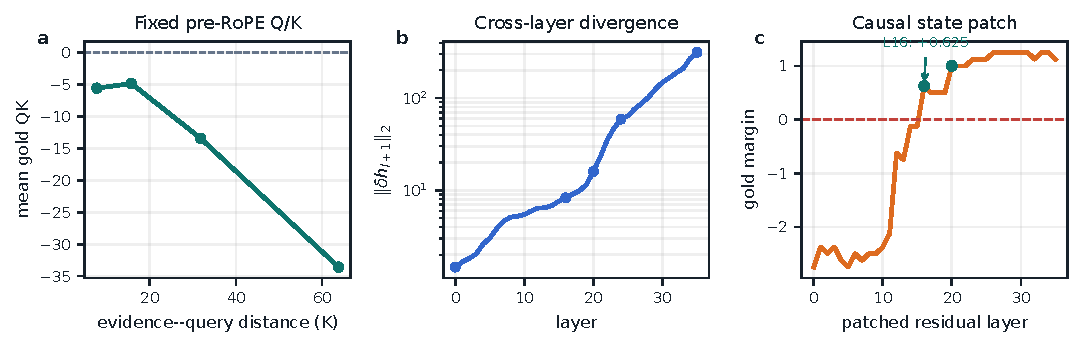
\includegraphics[width=\linewidth]{figures/mechanism_evidence.pdf}
  \caption{Mechanism evidence in Qwen3-8B.  \textbf{Left:} with identical
  pre-RoPE Q/K, the measured first-layer gold QK changes with distance; the
  64-pair analytic sum reconstructs it within $1.98\times10^{-3}$.
  \textbf{Middle:} a 64-token diagnostic perturbation creates a nonzero
  residual difference at layer 0 and the difference grows across depth.
  \textbf{Right:} replacing the failed run's residual input with the successful
  state at intermediate layers crosses the zero-margin decision boundary.}
  \label{fig:mechanism}
\end{figure}

\paragraph{Exact first-layer check.}
In a Qwen3-8B diagnostic with $d=128$, $\theta=10^6$, and YaRN scaling, we
freeze the same first-layer $\preq$ and $\prek$ and vary only their relative
positions.  Their norms and every pre-RoPE coordinate are identical across
the four runs.  Mean post-RoPE gold QK over 32 query heads changes from
$-5.588$ at distance 7,996 to $-33.586$ at 65,340
(\cref{fig:mechanism}).  Reconstructing the explicit rotation by summing
\cref{eq:pair-score} over all 64 pairs has maximum absolute error 0.00198.
This experiment does not claim that a negative layer-0 mean alone determines
the answer; it isolates the first causal input: phase can change a fixed
content score.

\subsection{Softmax converts score loss into weaker evidence writes}

For a gold token $g$ and competitor $c$ in the same softmax,
\begin{equation}
  \frac{a_g}{a_c}=\exp(s_g-s_c).
  \label{eq:attention-ratio}
\end{equation}
Reducing the relative gold score by one therefore multiplies its attention
advantage by $e^{-1}\approx0.368$.  More generally, differentiating softmax
gives
\begin{equation}
  \delta a_g
  \approx a_g\left(\delta s_g-\sum_j a_j\delta s_j\right).
  \label{eq:softmax-jacobian}
\end{equation}
The gold mass falls when its score changes less favorably than the current
attention-weighted mean competitor change.  Added filler can hurt through two
separable routes: it may change $s_g$ through phase, and its own exponentiated
scores enlarge the denominator.  Their effects interact multiplicatively,
but they are not the same mechanism.

The attention output written to the residual is
\begin{equation}
  o_l=W_{O,l}\sum_j a_{l,j}v_{l,j},
\end{equation}
with first-order change
\begin{equation}
  \delta o_l\approx W_{O,l}
  \left(\sum_j\delta a_{l,j}v_{l,j}
  +\sum_j a_{l,j}\delta v_{l,j}\right).
  \label{eq:value-write}
\end{equation}
The first term changes \emph{which} content is written; the second changes the
content vectors themselves.

\subsection{Later layers: phase-triggered state divergence}

For a pre-norm Transformer layer, write the exact real-valued update as
\begin{align}
  u_l&=h_l+\mathcal A_l(h_l;P,M),\\
  h_{l+1}&=u_l+\mathcal M_l(u_l),
\end{align}
where $P$ contains position information and $M$ the causal mask.  Comparing a
short trajectory $S$ with a longer trajectory $T$ gives the finite-difference
identity
\begin{equation}
  \delta h_{l+1}
  =\delta h_l+\delta\mathcal A_l+\delta\mathcal M_l.
  \label{eq:layer-difference}
\end{equation}
This is a vector identity: the three norms do not add because their pairwise
inner products matter.  In BF16, inserting the two actual rounding operators
replays all 36 layers with zero recorded error; the full expression appears in
\cref{app:layerwise}.

The score change in later layers has three first-order sources,
\begin{equation}
  \delta s_{l,j}\approx\frac{1}{\sqrt d}\left[
  \delta q_l^\top\Rope_{\Delta_j}k_{l,j}
  +q_l^\top\Rope_{\Delta_j}\delta k_{l,j}
  +q_l^\top\delta\Rope_{\Delta_j}k_{l,j}
  \right].
  \label{eq:three-score-sources}
\end{equation}
At layer 0, the final query embedding and hence $\delta q_0$ may be zero; the
phase and competing K/V sets still change attention.  From layer 1 onward,
\cref{eq:value-write} makes $\delta q_l$ and $\delta k_{l,j}$ nonzero.  The
proper description is therefore not ``RoPE rotates the same Q/K more at every
layer,'' but ``an initial phase perturbation sends the model onto a different
nonlinear state trajectory.''

\paragraph{Exact replay and causal patching.}
For the 143,424-to-143,488 diagnostic in \cref{fig:mechanism}, the query input
difference is zero, while the layer-0 attention and MLP differences have norms
0.542 and 1.293 and produce residual difference 1.466.  The residual difference
reaches 312.676 after layer 35.  Applying the real final RMSNorm and unembedding
reconstructs the target margin to $3.81\times10^{-6}$ and the gold probability
to $3.73\times10^{-8}$.  This exact replay is descriptive; causal evidence
comes from patching.  Copying the successful run's residual input into the
failed run at layer 16 changes the gold margin from $-2.75$ to $+0.625$; at
layer 20 it restores $+1.00$.  Thus the intermediate divergence is sufficient
to switch the decision.

